\section{Evaluation}
\label{sec:results}

% \subsection{Validation of eBPF processor}

% \begin{figure}[bth]
% \centering
% %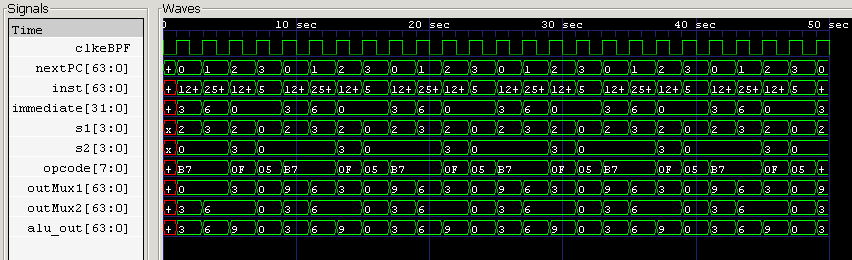
\includegraphics[width=1.\textwidth]{figures/07_fig02.png}
% 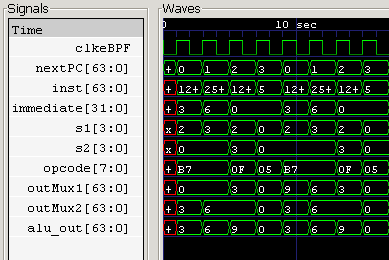
\includegraphics[width=1.\linewidth]{figures/07_fig02half.png}
% \caption{eBPF processor waveform instruction tests.}
% \label{fig:07_fig02}
% \end{figure}


% Firstly, for validation of the eBPF processor, we used the Altera Cyclone IV EP4CE115 platform. This FPGA has 114,480 logic cells, 50 MHz clock cycle and a set of memories (EEPROM, SRAM, Flash) with a storage capacity of 8 to 128 MB. We use the Altera platform with the aim of detecting and also correcting errors quickly before integrating the processor into the NetFPGA data path.


% % \begin{figure}[H]
% % \centering
% % \includegraphics[width=1.\textwidth]{imagens/06_fig10.png}
% % \caption{Forma de onda  processador eBPF.}
% % \label{fig:06_fig10}
% % \end{figure}




% Figure~\ref{fig:07_fig02} presents the generated waveform of the execution of an assembly program containing the following instructions: mov64, add, and ja (jump absolute). The first instruction to execute is an immediate mov64. In this instruction, register r2 receives the immediate value 3. The second instruction is also an immediate mov64. The register r3 receives the value 6. In the third instruction, the sum operation between r2 and r3 is executed. Both operations use the register file to read and write to the respective registers. Register r2, at the end of the sum operation, has value 9 and stores it in the register file. The last instruction is a jump to the beginning of the code, the program counter goes to zero, initializing its operations. The last line in the Figure (alu\_out), represents the output of the ALU according to each instruction.


% With the exception of the call instruction, as explained earlier, the eBPF processor has been synthesized and tested for all eBPF instructions on an Intel Altera platform. Then, the same processor was synthesized in Xilinx Vertex-II Pro 50 FPGA. Xilinx software synthesized all instructions except multiplication, division, and remainder instructions. In practice, these instructions are not widely used on a switch. In addition, these instructions with the power of 2 can be executed with the operations shift left, shift right, and logical operator and, respectively. We believe that a newer version of NetFPGA can accept the synthesis of these instructions. The project with the inclusion of these instructions, described in Verilog, is correctly synthesized in the Intel Altera FPGA development environment.

%Na figura~\ref{fig:06_fig11}

The eBPFlow was synthesized in the NetFPGA SUME and occupied 58\% of logical slice and 27\% of the register slice. The maximum frequency is 88.83 MHz (cycle of 11.25 ns).


\subsection{Experiments} 
\label{sec:experiments}

% \begin{figure}[ht]
% \centering
% 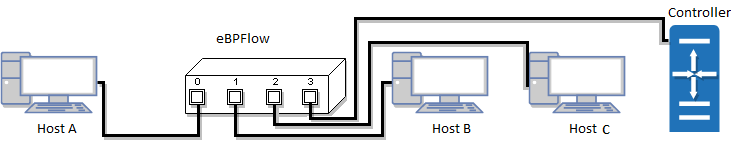
\includegraphics[width=1.\linewidth]{figures/07_fig03-3hosts.png}
% \caption{Topology of the experiments.}
% \label{fig:07_fig03}
% \end{figure}

\begin{figure}[htb]
\centering
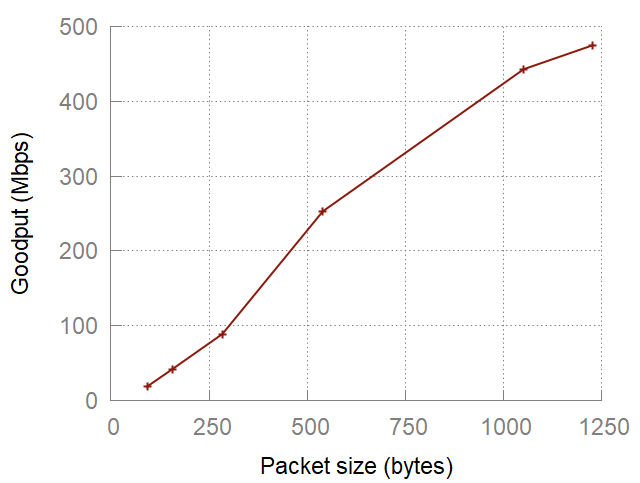
\includegraphics[width=1.\linewidth]{figures/goodputxbytes.png}
%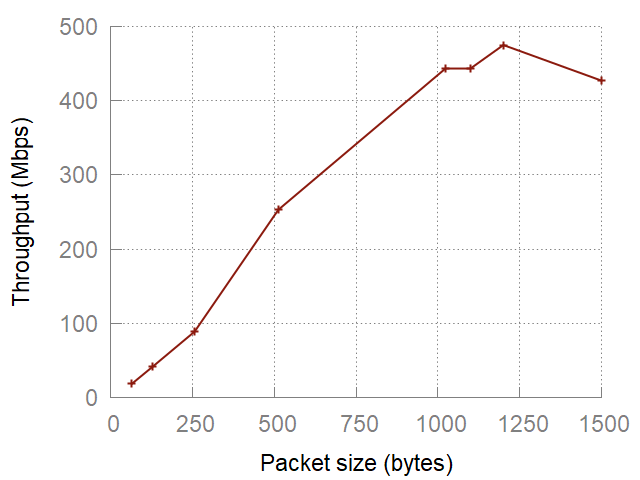
\includegraphics[width=1.\linewidth]{figures/throughputxbytes.png}
\caption{Goodput per packet size.}
\label{fig:07result}
\end{figure}

% Figure~\ref{fig:07_fig03} presents the topology of the experiments. The NetFPGA has 4 ports. The switch interconnects three host computers and also connects to the controller.

% We developed C language applications. The code is compiled with LLVM 3.9 for the eBPF big endian platform.
% The LLVM compiler generates an executable in the executable and link format (ELF).
% The objcopy tool extracts the instruction set from the .text segment of the elf file.
% The controller installs this segment into eBPFlow.

The first application forwards frames from one interface to another. There is no learning involved, the output ports are hard-coded. Using the iperf tool, UDP connections are created between terminals A and B. Figure~\ref{fig:07result} shows the UDP goodput per packet size. This experiment evaluates what is the maximum obtained goodput.

The second example is an IPv4 router.
When eBPFlow receives a frame, it checks if the frame is an Ethernet frame and if it contains an IPv4 packet. It extracts the IPv4 destination and searches the TCAM for the output port.
The available actions are to forward the packet or drop it.
Figure~\ref{fig:IPv4routerresult} shows the goodput for UDP flow with packets of 1472 bytes.

\begin{figure}[htb]
\centering
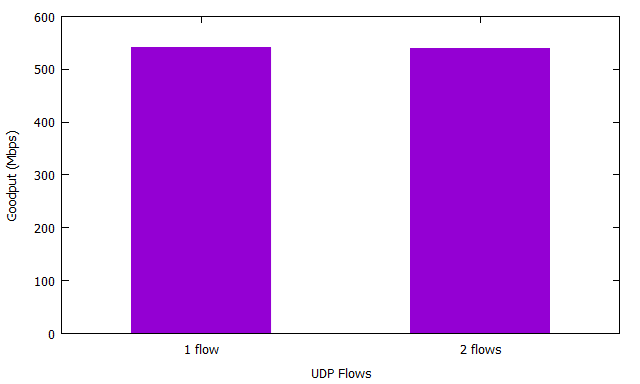
\includegraphics[width=1.\linewidth]{figures/ipv4goodput.png}
%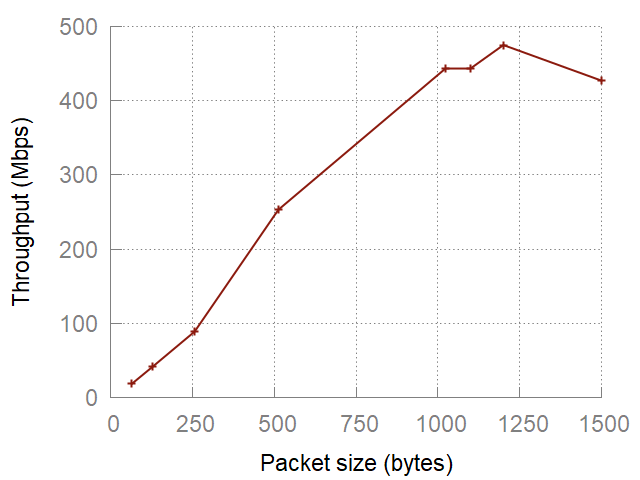
\includegraphics[width=1.\linewidth]{figures/throughputxbytes.png}
\caption{UDP Goodput for IPv4 router.}
\label{fig:IPv4routerresult}
\end{figure}

% \begin{table}[htb]
% \centering
% \begin{tabular}{|c|c|}
% \hline
% Number of Flows & Goodput (Mbps) \\
% \hline
% 1 & 541 $\pm$ 4.9 \\
% \hline
% 2 & 539 $\pm$ 13.99 \\
% \hline
% \end{tabular}
% \caption{UDP Goodput for IPv4 router.}
% \label{tab:IPv4routerresult}
% \end{table}


The third application is an L2 learning switch.
The advantage of a protocol-independent switch is that it only needs to parse the frame header fields for the protocols defined by the programmer. In this example, the parser only needs to parse Ethernet headers while protocol-dependent switch would process other frame or packet header fields. CAM (exact-match) lookup table stores the Ethernet MAC address and the input port. 
For each input frame, if the source address is unicast, the code can self-populate the lookup table by updating it.
This second advantage can reduce network traffic, latency, and CPU controller overhead.
Using the destination MAC, the output port is searched.
If there is an entry, then the packet is forwarded otherwise there are two options. It can be flooded or sent to the controller. In this experiment, we opted to flood.


The code is installed through the NetFPGA register interface.
The time to read or write one register in this interface is 500 us.
Each eBPF instruction (64 bits) utilizes two registers (32 bits).
To start the code installation, it requires 2 write operations.
Thus, the time to install a code is given by:\\
Time to install code $=$ (number of instructions+2) $* 500 us * 2.$ 

In the last experiment, eBPFlow starts as IPv4 router. During runtime, we install the learning switch. This experiment validates the system by showing that the switch executes these instructions for each received packet, allowing a data plane with dynamic parse, matching, and actions at run time with zero downtime.

\textbf{ChaCha:} 
ChaCha20~\cite{rfc8439} network function is a
stream cipher used in Transport Layer Security (TLS) by Google for symmetric
encryption~\cite{google-chacha}.
ChaCha20 cannot be implemented in the P4 switch.
The number after ChaCha indicates how many rounds to apply the cipher over the data.
We tried to implement it on the Netronome Agilio CX 1x40 Gbps SmartNIC but it can only support up to eight rounds. Netronome expressiveness can be categorized as eBPF-verifier. It requires the verifier and loop unrolling, which increases the number of instructions and thus does not fit in the smartNIC memory instruction.
But, \system is able to execute ChaCha20.




\subsection{Power}

When idle, the NetFPGA consumes 16 W.
When eBPFlow is loaded, the power consumption is 22 W independent of the packet rate or what programming is running.
On the other hand, an idle CPU already consumes 85 W.
Thus, eBPFlow saves power in comparison to software packet processing.


